
\chapter{Mise en \oe{}uvre de \PpFf}
\label{implementation.chap}


Ce chapitre décrit la fa\c{c}on dont \TT{PpFf} est impl\'ement\'e. 
%
De fa\c{c}on g\'en\'erale, la mise en \oe{}uvre utilise la biblioth\`eque \TT{FastFlow}, et ce en h\'eritant et \'etendant plusieurs de ses classes.

Ce chapitre est divis\'e en trois sections.
%
La premi\`ere section d\'ecrit les diff\'erents éléments composant la biblioth\`eque \TT{PpFf}. La deuxi\`eme section examine comment la parall\'elisation du flux est r\'ealis\'ee. La derni\`ere section pr\'esente quelques exemples d\'ecrivant comment un programme \PpFf{} est compil\'e et ex\'ecut\'e.


\section{Les \'el\'ements de \TT{PpFf}}

\begin{figure}
\centering
         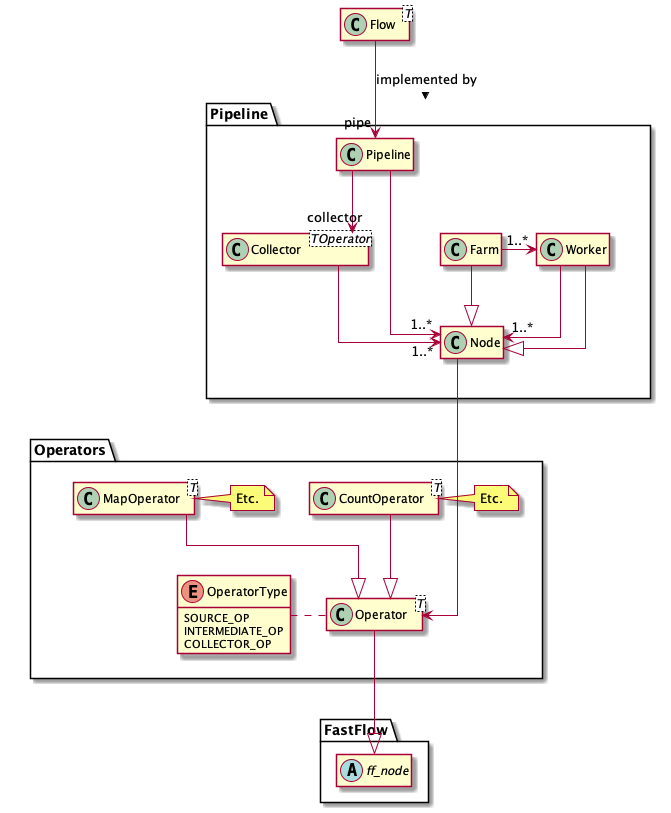
\includegraphics[width=1.0\textwidth]{Figures/vueEnsemble.png}
      \caption{Les principaux éléments (classes et paquetages) de \TT{PpFf}.}
       \label{All.fig}
\end{figure}

La biblioth\`eque \TT{PpFf} est compos\'ee de plusieurs modules qui permettent de g\'erer les flux de traitement de donn\'ees. Une vue d'ensemble de ces modules est illustr\'ee dans la figure~\ref{All.fig}.

\begin{itemize}

\item Le point d'entr\'ee de \ppff\ est la classe \TT{Flow}, avec laquelle interagissent les d\'eveloppeurs pour cr\'eer des flux de traitement. Toutes les op\'erations de traitement d'un flux de \TT{PpFf} sont li\'ees aux m\'ethodes expos\'ees par cette classe. 

\item Le c\oe{}ur de la mise en \oe{}uvre de \TT{PpFf} est le module \TT{Pipeline}. La cr\'eation et l'ex\'ecution d'un flux sont g\'er\'ees par celui-ci, qui construit tout d'abord une représentation intermédaire, et qui génère ensuite un graphe de n\oe{}uds FastFlow.

\item  Le module \TT{Operators} regroupe tous les op\'erateurs d\'efinis dans \TT{PpFf}. Expos\'es \`a l'utilisateur par le biais de l'\TT{API} de \TT{PpFf}, ces op\'erateurs permettent de traiter les donn\'ees de diverses façons.

\item Le dernier module, \TT{FastFlow}, est la biblioth\`eque au–dessus de laquelle \TT{PpFf} est impl\'ement\'e.


\end{itemize}

\subsection{Flow}
\label{flow.chap}

\begin{figure}
\centering
     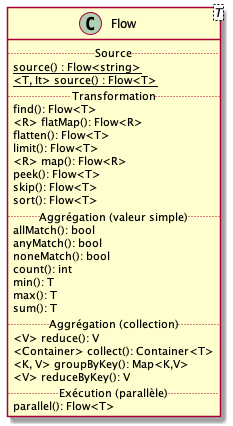
\includegraphics[width=0.5\textwidth]{Figures/flow-details.png}
      \caption{Les m\'ethodes export\'ees par l'API de \TT{PpFf}.}
       \label{Flow.fig}
\end{figure}



La classe \TT{Flow} est celle qui définit l'\TT{API} de la biblioth\`eque \TT{PpFf}, l'interface avec laquelle interagit le d\'eveloppeur. La figure~\ref{Flow.fig} --- qui reprend la figure~\ref{MethodesAPI.fig} --- pr\'esente les diverses m\'ethodes export\'ees par \TT{PpFf}. Selon le type du résultat export\'e par l'\TT{API}, les m\'ethodes sont divis\'ees en plusieurs groupes : Source, Transformation, Agr\'egation (valeur simple ou collection) et Ex\'ecution (parallèle).

\begin{itemize}

\item Le premier groupe, Source, est le groupe de méthodes (statiques) qui permettent de créer un flux de donn\'ees. Ce sont des m\'ethodes qui fournissent les donn\'ees initiales pour un flux. Sans un appel \`a une telle m\'ethode, un flux ne peut pas exister. 

\item Le deuxi\`eme groupe, Transformation, est composé des m\'ethodes qui retournent une r\'ef\'erence vers un objet \TT{Flow}. C'est ce m\'ecanisme permet d'encha\^iner les m\'ethodes de l'\TT{API}.

\item Le troisi\`eme groupe, Agr\'egation, est divis\'e en deux sous-groupes, selon le type de r\'esultat produit : valeur simple --- les m\'ethodes retournant une valeur simple, habituellement un scalaire (par ex., r\'esultat bool\'een ou entier) et collection --- les m\'ethodes retournant une collection.

\item Le quatrième et dernier groupe, Exécution, comporte une seule m\'ethode. Cette m\'ethode modifie le comportement d'ex\'ecution du flux. Lorsqu'elle est ajout\'ee au  \TT{pipeline}, toutes les op\'erations suivant cette m\'ethode seront ex\'ecut\'ees en parall\`ele, en utilisant les instances d'un  \TT{farm}.

L'\TT{API} de \TT{PpFf} permet d'appliquer plusieurs op\'erations les unes à la suite des autres sur une collection de donn\'ees. Ceci est possible en encha\^inant les m\'ethodes (\emph{method chaining}). Les m\'ethodes de l'\TT{API} peuvent \^etre enchain\'ees tant qu'elles retournent une r\'ef\'erence \`a \TT{Flow}. Lorsqu'une m\'ethode retourne une valeur, une valeur simple ou une collection, le traitement est alors ex\'ecut\'e. 

\end{itemize}


\begin{lstlisting}[
label={source.c++},
language=c++,
gobble=4,
caption={Des extraits (squelette) de la classe \TT{Flow} avec la variable d'instance \TT{pipe} et le code de la m\'ethode statique \TT{soure}.},
frame=single,
float]
    class Flow {

    public:
        static Flow& source(const std::string& path) {
            Flow* flow = new Flow();
            flow->pipe.addNodes<LinesFromFileOperator>(1, path);

            return *flow;
        }

        // ... Autres methodes....
        // ... Voir autres listings pour des exemples...

    private:
        Pipeline pipe;
    };
\end{lstlisting}


\begin{lstlisting}[
label={map.c++},
language=c++,
gobble=7,
caption={Le code de la m\'ethode \TT{map}, m\'ethode qui fait partie du groupe \TT{Transformation} de la classe \TT{Flow}.},
frame=single,
float]
        template < typename In, typename Out >
        Flow& map(std::function<Out*(In*)> const& taskFunc) {
            pipe.addNodes<MapOperator<In, Out>>(pipe.nbWorkers(), taskFunc);

            return *this;
        }
\end{lstlisting}


\begin{lstlisting}[
label={count.c++},
language=c++,
gobble=7,
caption={Le code de la m\'ethode \TT{count}, m\'ethode qui fait partie du groupe \TT{Agr\'egation} de la classe \TT{Flow}.},
frame=single,
float]
        unsigned int count() {
            pipe.addNodes<CountOperator<int>>(pipe.nbWorkers());
            pipe.run();

            return pipe.value<CountOperator<int>, int>();
        }
\end{lstlisting}


L'\TT{API} de \TT{PpFf} est mise en œuvre par le module \TT{Pipeline}. Ce dernier s'occupe de la cr\'eation et de l'ex\'ecution du flux. Les listings~\ref{source.c++},~\ref{map.c++} et~\ref{count.c++} pr\'esentent le code de trois m\'ethodes de l'\TT{API} appartenant \`a trois groupes diff\'erents: \TT{Source}, \TT{Transformation} et \TT{Agrégation}. L'attribut \TT{pipe} utilisée dans chaque m\'ethode est une instance de la classe \TT{Pipeline}, objet qui cr\'ee et ajoute les op\'erateurs dans le pipeline associ\'e au flux en appelant la m\'ethode \TT{addNodes} --- voir ci-bas. 

Une m\'ethode statique \TT{source}, comme dans le listing~\ref{source.c++}, est toujours la premi\`ere m\'ethode appelée, pour créer le flux de traitement. Cette m\'ethode a un double r\^ole : elle cr\'ee un objet \TT{Flow} puis fournit les donn\'ees initiales du flux de donn\'ees. Le listing~\ref{map.c++} pr\'esente la m\'ethode \TT{map}, qui appartient au groupe \TT{Transformation}, et qui ne fait qu'ajouter une série de n\oe{}uds au pipeline de traitement. Ces deux m\'ethodes, \TT{source} et \TT{map}, retournent un objet \TT{Flow}, ce qui permet le chainage de méthodes. La troisi\`eme m\'ethode, \TT{count}, qui appartient au groupe \TT{Agr\'egation}, retourne une valeur enti\`ere
---
\TT{int}, tel que sp\'ecifi\'e dans le deuxi\`eme param\`etre générique de la m\'ethode \TT{pipe.value()}
---
valeur qui indique le nombre d'\'el\'ements du flux. Plus exactement, cette valeur est obtenue (avec \TT{value()}) après avoir ex\'ecuté le traitement associé au flux, ce qui se fait avec la m\'ethode \TT{pipe.run()}.

\subsection{Pipeline}

\begin{figure}
\centering
         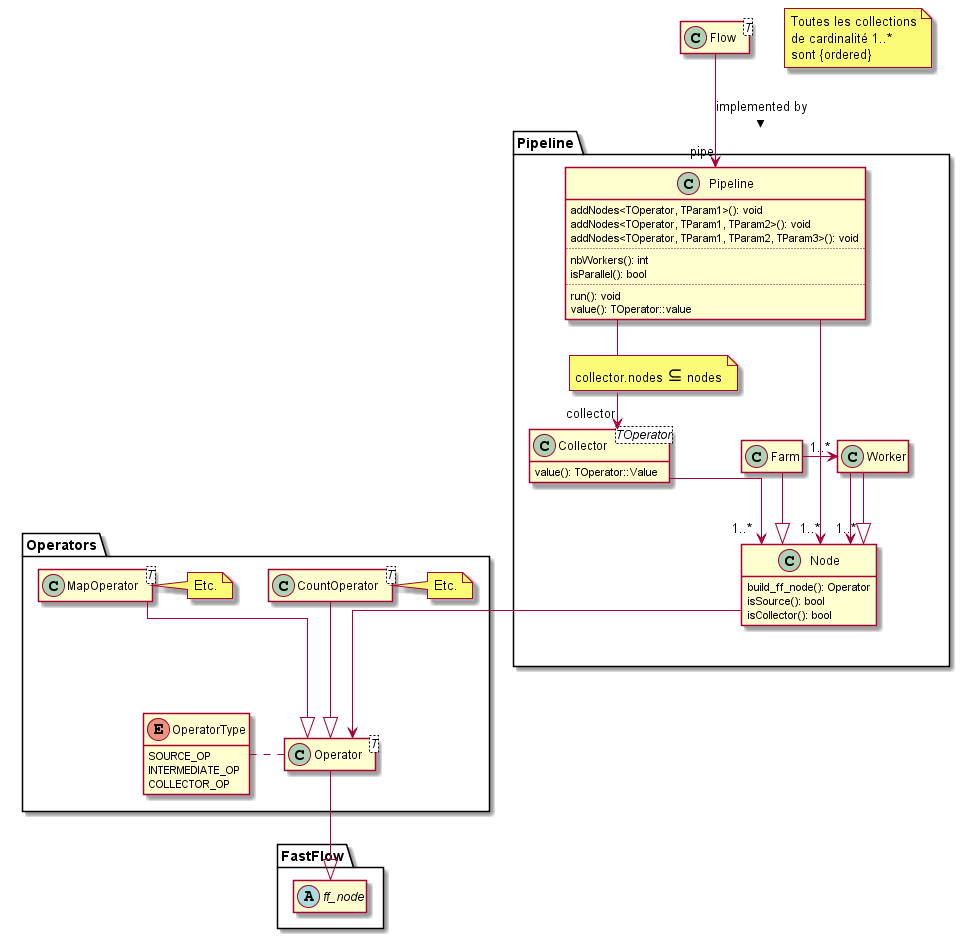
\includegraphics[width=0.8\textwidth]{Figures/pipeline.png}
      \caption{Un diagramme UML des éléments pour un \TT{Pipeline} de \ppff.}
       \label{pipeline.fig}
\end{figure}

\TT{PpFf} est impl\'ement\'e au-dessus de la biblioth\'eque \TT{FastFlow}. Plus précisément, \TT{PpFf} construit tout d'abord une repr\'esentation interm\'ediaire, puis g\'en\`ere ensuite un graphe de n\oe{}uds \TT{FastFlow}. Toutes les classes n\'ecessaires pour construire une telle structure interm\'ediaire sont group\'ees dans le module \TT{Pipeline}, tel qu'illustr\'e dans le diagramme de classes de la figure~\ref{pipeline.fig}.

La classe principale de ce module, la classe avec le m\^eme nom que le module, est la classe \TT{Pipeline}. Une instance de cette classe repr\'esente une cha\^ine de traitement. Plus pr\'ecis\'ement, \TT{Pipeline} est l'impl\'ementation du flux \TT{Flow} d\'ecrit dans la sous-section~\ref{flow.chap}. Un objet \TT{Pipeline} est compos\'e d'une ou plusieurs instances de la classe \TT{Node}. Un \TT{Node} peut \^etre un \TT{Pipeline}, un \TT{Worker} ou un \TT{Farm}. Les classes \TT{Worker} et \TT{Farm} sont utilis\'ees pour cr\'eer les instances parall\`eles d'un \TT{farm} — voir plus bas. Les instances \TT{Node} sont ajout\'ees au flux en appelant la m\'ethode \TT{addNodes} de la classe \TT{Pipeline}. En fonction de type de parall\'elisme (de flux, Sect.~\ref{ParallelismeDuFlux.sect} ou de donn\'ees, Sect.~\ref{ParallelismeDeDonnees.sect}), un objet \TT{Pipeline} peut \^etre compos\'e d'instances de \TT{Node} ou  de \TT{Farm}. Lorsqu'une instance de \TT{Farm} est ajout\'ee au {pipeline}, le flux est divis\'e en sous-flux --- appel\'es les instances parall\`eles d'un \TT{farm} --- où chaque sous-flux est une instance de la classe \TT{Worker}. Un objet \TT{Worker} peut, \`a son tour, \^etre un objet \TT{Node} ou un objet \TT{Pipeline}.

La structure ainsi cr\'e\'ee sera parcourue lorsque le dernier \TT{Node} ajout\'e au \TT{pipeline} est un collecteur (identifi\'e \`a l'aide de la m\'ethode \TT{isCollector} de cette classe). L'ex\'ecution du \TT{pipeline} –-- fait par l'appel de la m\'ethode \TT{run} --- implique des appels \`a la m\'ethode \TT{build\_ff\_node()} de chaque \TT{Node} de la structure intermédiaire pour construire le graphe \TT{FastFlow} appropri\'e. Ce dernier, compos\'e des objets de type \TT{ff\_pipeline}, \TT{ff\_node} et \TT{ff\_farm} correspondant aux objets \TT{Pipeline}, \TT{Node} et \TT{Farm} de \TT{PpFf}, est ex\'ecut\'e directement à l'aide de la méthode appropriée d'un pipeline FastFlow (\TT{run\_and\_wait\_end()}).

Le r\'esultat du traitement est retourn\'e au \TT{Pipeline} par l'intermédiare de la méthode \TT{value()} de l'objet \TT{Collector}. Si le traitement se fait en parallèle en utilisant les instances d'un \TT{farm}, l'objet \TT{Collector} du pipeline combine les r\'esultats partiels obtenus de chacun des sous-flux.



\subsection{Operators}

\begin{figure}
\centering
         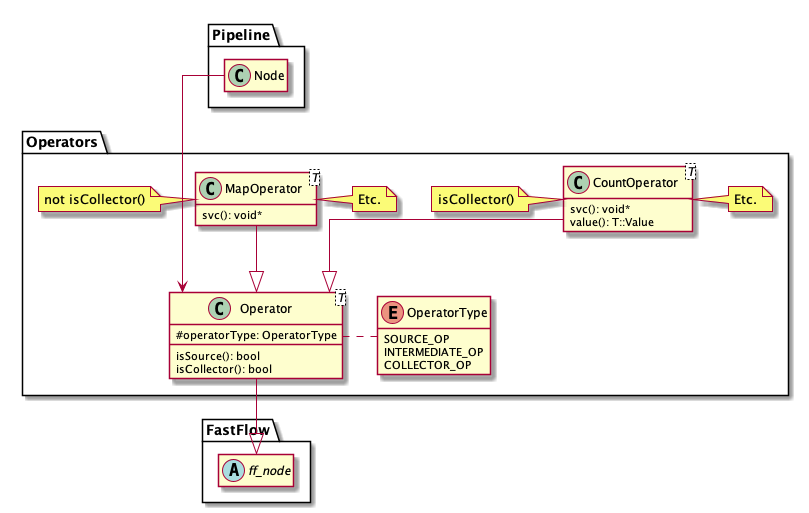
\includegraphics[width=1.0\textwidth]{Figures/operators-details.png}
      \caption{Un diagramme UML des \TT{Operators} de \ppff.}
       \label{operators.fig}
\end{figure}


Dans la terminologie de \TT{PpFf}, chaque m\'ethode expos\'ee par l'interface de \ppff\ repr\'esente une op\'eration et chaque op\'eration est impl\'ement\'ee par un op\'erateur, un objet provenant d'une sous-classe de la classe \TT{Operator}. Plus pr\'ecisément, les op\'erateurs repr\'esentent les \'etapes dans la chaine de traitement de donn\'ees. Tel qu'illustré dans la figure~\ref{operators.fig}, les classes pour les divers op\'erateurs h\'eritent de la classe de base, \TT{Operator}. 
%
Notons que sur cette figure, pour alléger le diagramme, seules deux sous-classes, \TT{MapOperator} et \TT{CountOperator}, ont été indiqu\'ees, les autres \'etant implicites, via le <<Etc.>>.
%

Ces divers opérateurs peuvent \^etre regroupés en trois cat\'egories : \emph{source}, \emph{interm\'ediaire} et \emph{collecteur}.
%
Un objet \TT{Pipeline} complet est compos\'e d'un op\'erateur source, de z\'ero ou plusieurs op\'erateurs interm\'ediaires et d'un op\'erateur collecteur. 

L'op\'erateur source est le premier op\'erateur ajout\'e dans le flux~; sans un tel op\'erateur, aucun traitement ne peut avoir lieu puisqu'il n'y aurait pas de données à traiter. Les deux op\'erateurs qui font partie de ce groupe sont \TT{SourceOperator} et \TT{LinesFromFileOperator}.

Les op\'erateurs interm\'ediaires, tels que \TT{FindOperator}, \TT{FlatMapOperator}, \TT{FlatOperator}, \TT{LimitOperator}, \TT{MapOperator}, \TT{PeekOperator} ou \TT{SkipOperator}, sont des op\'erateurs qui traitent chaque \'el\'ement du flux de fa\c{c}on ind\'ependante. Autre point important~: les op\'erateurs interm\'ediaires n'effectuent aucun traitement tant qu'un op\'erateur collecteur n'est pas ajout\'e au \TT{pipeline}. 

Le plus nombreux groupe d'op\'erateurs est celui des collecteurs, qui réunit les op\'erateurs suivants : \TT{AllMatchOperator}, \TT{AnyMatchOperator}, \TT{NoneMatchOperator}, \TT{GroupByKeyOperator}, \TT{MaxOperator}, \TT{MinOperator}, \TT{ReduceOperator}, \TT{CollectorOperator}, \TT{SumOperator}, \TT{CountOperator}, \TT{ReduceByKeyOperator} et \TT{SortOperator}. Un op\'erateur de type collecteur est toujours le dernier ajout\'e au \TT{pipeline}. L'ajout de cet op\'erateur entra\^ine l'ex\'ecution du traitement spécifié par les opérateurs du pipeline. La valeur r\'esultante du traitement est conserv\'ee en interne par chaque op\'erateur collecteur. C'est cette valeur qui va \^etre retourn\'ee au \TT{Pipeline} par un appel à \TT{value()}.

La fonctionnalit\'e sp\'ecifique \`a chaque op\'eration du \TT{pipeline} est impl\'ement\'ee par la m\'ethode \TT{svc} de chaque op\'erateur. Comme on peut le voir dans la figure~\ref{operators.fig}, un \TT{Operator} h\'erite de la classe \TT{ff\_node} de \TT{FastFlow}. De cette fa\c{c}on, lorsque le graphe FastFlow est exécuté, c'est la méthode \TT{svc} de chaque op\'erateur qui est appel\'ee. C'est ce qui permet de spécifier la fonctionnalit\'e spécifique à chaque opérateur 








\section{\'Ex\'ecution parall\`ele avec parall\'elisme de flux ou de donn\'ees}

\TT{PpFf} permet aux programmeurs de composer des morceaux de code s\'equentiel --- des fonctions ou expressions lambdas --- et d'ex\'ecuter le tout en parall\`ele, et ce à l'aide de deux formes de parallélisme~:
parall\'elisme de flux et parall\'elisme de donn\'ees.
%
L'objectif de cette section est de d\'ecrire la façon dont ces deux formes de parall\'elisme sont impl\'ement\'es en \TT{PpFf}. 

\subsection{Parall\'elisme de flux}
\label{ParallelismeDuFlux.sect}

Le parall\'elisme de flux consiste \`a ex\'ecuter plusieurs \'etapes d'un traitement s\'equentiel en parall\`ele en leur faisant traiter des donn\'ees diff\'erentes. Les donn\'ees se succ\`edent ainsi les unes aux autres dans les diff\'erentes \'etapes.

Dans \TT{PpFf}, une {\'etape} est cr\'e\'ee lorsqu'une m\'ethode de l'interface de \TT{PpFf} est ajout\'ee au \emph{pipeline} par le cha\^inage de m\'ethodes.

\`A noter que ce type de parall\'elisme est appliqu\'e par d\'efaut dans notre biblioth\`eque. 
%
Ce fonctionnement permet de parall\'eliser des traitements avec des d\'ependances entre les donn\'ees sans avoir recours \`a des synchronisations \emph{explicites} par le programmeur. 

\goodbreak
\begin{samepage}
Un flux compos\'e de $n$ {étapes}, o\`u la $i^{\grave e}$ étape ex\'ecute une op\'eration $O_i$, peut \^etre vu sous la forme d'une composition s\'equentielle d'op\'erations sur les \'el\'ements d'entr\'ee comme suit, o\`u $O(x)$ repr\'esente le traitement global d'un des \'el\'ements $x$ du flux de données~: 
%
\[
	O(x) = O_n( \ldots (O_k( \ldots O_1(x)) \ldots ) \ldots ));
\]
\end{samepage}


\begin{figure}

\centering
     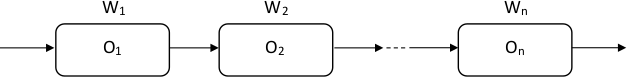
\includegraphics[width=0.9\textwidth]{Figures/ParallelismeDuFlux.png}
      \caption[Une repr\'esentation graphique du parall\'elisme de flux en \ppff.]{Une repr\'esentation graphique du parall\'elisme de flux pour une d\'ecomposition en $n$. Les op\'erations $O_1, O_2, \ldots, O_n$ sont ex\'ecut\'ees de fa\c{c}on parall\`ele dans diff\'erents fils d'ex\'ecution représentés par $W_1, W_2, \ldots, W_n$ ($W$ pour \emph{$W$orker}).}
       \label{ParallelismeDuFlux.fig}
\end{figure}


Si on note par $W_i$ le fil d'ex\'ecution (\emph{thread}) associ\'e à la $i^{\grave e}$ {étape}, alors
le parall\'elisme de flux du pipeline peut \^etre repr\'esent\'e par un graphe lin\'eaire de $n$ travailleurs. Chaque travailleur correspond \`a une op\'eration sp\'ecifique $O_i$. La figure~\ref{ParallelismeDuFlux.fig} montre la repr\'esentation graphique du parall\'elisme de flux dans un tel pipeline. Signalons que cette approche n'acc\'el\`ere pas le calcul d'un \'el\'ement donné du flux, qui doit parcourir toutes les étapes; par contre, elle peut am\'eliorer \emph{le d\'ebit de sortie} si les opérations $O_i$ sont complexes.

\subsection{Parall\'elisme de donn\'ees}
\label{ParallelismeDeDonnees.sect}

Le parall\'elisme de donn\'ees impl\'ement\'e dans \TT{PpFf}  consiste \`a r\'epliquer une op\'eration sur un ensemble de travailleurs identiques. Autrement dit, il vise \`a effectuer un traitement identique sur un ensemble de donn\'ees ind\'ependantes les unes des autres. 
%
Dans notre impl\'ementation de \PpFf, le parall\'elisme de donn\'ees est mis en \oe{}uvre avec les \emph{Task Farm} de \TT{FastFlow}.


D\'ecrit \`a la section~\ref{farm.sect}, un \emph{Task Farm} est compos\'ee de trois entit\'es : un \emph{Emitter}, plusieurs instances de travailleurs (\emph{workers}), et un \emph{Collector}. Par d\'efaut, dans \PpFf{}, les \'el\'ements sont r\'epartis par un \emph{Emitter} aux divers travailleurs selon une politique \emph{round robin}.%
%
\footnote{Politique \emph{round robin}~: approche d'ordonnancement pour r\'epartir la charge du travail entre des \emph{threads}, avec une file d'attente circulaire. Cf.~\url{https://fr.wikipedia.org/wiki/Round-robin_(informatique)}.} 
%
Les travailleurs re\c{c}oivent les \'el\'ements d'entr\'ee et appliquent sur chacun l'op\'eration sp\'ecifi\'ee au pr\'ealable par l'utilisateur. Les r\'esultats sont ensuite envoy\'es vers le \emph{Collector} charg\'e de les collecter --- i.e., de les combiner --- puis de les transmettre sur le flux de sortie.

Dans \TT{FastFlow} un \emph{Task Farm} est cr\'e\'e en instanciant la classe \TT{ff\_farm}. Cette classe correspond \`a la classe \TT{Farm} du module \TT{Pipeline}. Lorsqu'une instance de \TT{Farm} est ajout\'ee au \emph{pipeline}, le flux est divis\'e en sous-flux --- appel\'es les instances parall\`eles d'un \TT{farm}. Ceci est possible en utilisant la m\'ethode \TT{parallel} de l'API de \TT{PpFf}. Le nombre de sous-flux ainsi cr\'e\'es d\'epend de la valeur sp\'ecifi\'ee en param\`etre pour cette m\'ethode.  

Dans \TT{PpFf}, les \'el\'ements du flux sont trait\'es dans l'ordre d'arriv\'ee selon le principe \emph{FIFO}. La collection de plusieurs r\'esultats \`a l'aide de cette approche r\'esulte dans un flux sans ordre sur ses \'el\'ements. En effet, le \emph{Collector} transmet les \'el\'ements au flux de sortie dans l'ordre d'arriv\'ee. \'Etant donn\'e que plusieurs flux ind\'ependants sont impliqu\'es, cet ordre ne peut pas \^etre pr\'ed\'etermin\'e. Si le respect d'un  ordre sp\'ecifique est requis, l'utilisateur de l'API peut ajouter une op\'eration qui produit cet ordre. Par exemple, la m\'ethode \TT{sort} de l'API (cf.~l'annexe~\ref{methodes-api.ann}), effectue le tri des \'el\'ements du flux selon l'ordre sp\'ecifi\'e par la fonction \TT{compare} envoy\'e en param\`etre.

\begin{figure}

\centering
     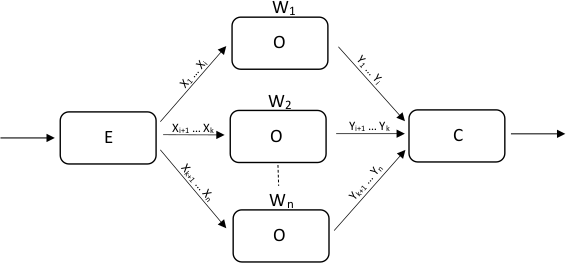
\includegraphics[width=0.9\textwidth]{Figures/DataParallelisme.png}
      \caption[Une repr\'esentation graphique du parall\'elisme de donn\'ees en \ppff.]{Une repr\'esentation graphique du parall\'elisme de donn\'ees. La m\^eme op\'eration~$O$ est ex\'ecut\'ee par les $n$ travailleurs $W_1, W_2,\ldots, W_n$ ($W$ pour \emph{$W$orker}). Les \'el\'ements de donn\'ees sont r\'epartis entre les travailleurs par l'\'emetteur $E$ ($E$\emph{mitter}) puis les divers r\'esultats sont combin\'es par le collecteur $C$ ($C$\emph{ollector}).}
       \label{DataParallelisme.fig}
\end{figure}


L'impl\'ementation parall\`ele de ce mod\`ele peut \^etre
exprim\'ee sous la forme d'un ensemble de~$n$ travailleurs $W_1, W_2,\ldots, W_n$ qui
appliquent une op\'eration $O$ sur les divers \'el\'ements~$X = \{x_1, \ldots, x_k\}$ apparaissant dans
le flux d'entr\'ee pour produire en sortie un ensemble d'\'el\'ements~$Y = \{y_1, \ldots, y_k\}$, o\`u $y_i = O(x_i)$.
%
Les divers \'el\'ements $x_i~(i=1, \ldots, k)$ sont r\'epartis entre
les travailleurs $W_j~(j=1, \ldots, n)$ d'une fa\c{c}on
ind\'etermin\'ee, qui d\'epend notamment de la vitesse de traitement
de chaque $x_i$.
%

La figure~\ref{DataParallelisme.fig} montre une repr\'esentation graphique du parall\'elisme de donn\'ees, o\`u la m\^eme op\'eration $O$ est ex\'ecut\'ee par les travailleurs $W_1, W_2,\ldots, W_n$. 

Il est possible de sp\'ecifier en param\`etre le nombre de travailleurs \`a utiliser pour l'ex\'ecution parall\`ele. Si ce param\`etre n'est pas sp\'ecifi\'e, un seul travailleur est activ\'e. Permettre ainsi d'augmenter le nombre de travailleurs fait en sorte qu'on peut augmenter le d\'ebit du traitement des donn\'ees si appropri\'e, c'est-\`a-dire, augmenter le nombre de donn\'ees qui peuvent \^etre trait\'ees en un temps donn\'e si le nombre de c\oe{}urs ou processeurs le permet.




\section{Impl\'ementation de \TT{PpFf} avec \TT{FastFlow} : quelques exemples}

Cette section d\'ecrit le mod\`ele d'ex\'ecution de \TT{PpFf} via \TT{FastFlow} \`a l'aide du code source de trois petits exemples. Ces exemples illustrent, \`a l'aide de diagrammes de classes, la structure de la représentation intermédiaire et la relation entre cette représentation intermédiaire et le graphe \TT{FastFlow} associé.


\subsection{Exemple~1~: Un flux simple avec uniquement une source et un collecteur} 


\begin{lstlisting}[
label={objets1.c++},
language=c++,
gobble=4,
caption={Le code source d'un flux pour trouver le maximum d'une collection de données.},
frame=single,
float]
    std::vector<int> elems = {0, 1, 2, 3, 4, 5, 6, 7, 8, 9};

    int currentResult =
        Flow
        ::source<int>(elems.begin(), elems.end())
        .max<int>();
\end{lstlisting}

Illustr\'e dans le listing~\ref{objets1.c++}, le premier exemple analys\'e ne comporte que deux op\'erations :

\begin{itemize}
\item \TT{source}, la méthode (statique) qui g\'en\`ere un flux s\'equentiel de nombres entiers \`a partir d'un conteneur (en \TT{vector}); 
\item \TT{max}, la méthode (d'instance) qui trouve l'\'el\'ement maximum du flux. 


\end{itemize}



\begin{figure}
\centering
         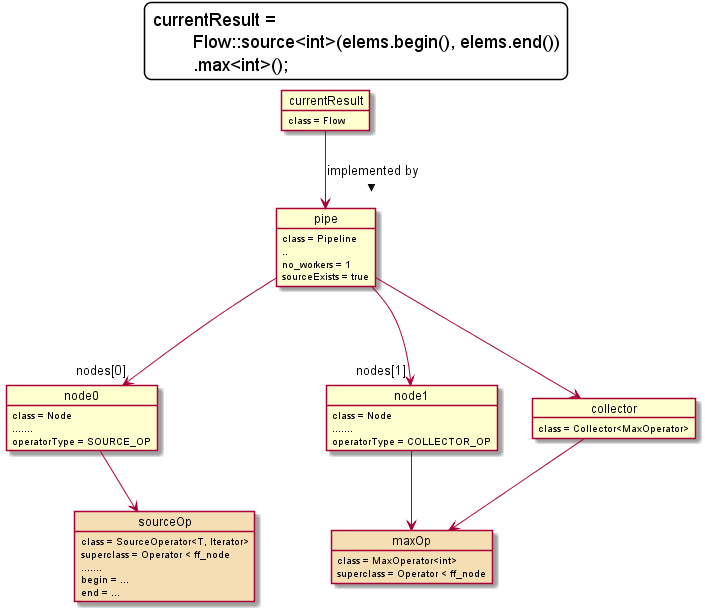
\includegraphics[width=0.66\textwidth]{Figures/objets1-ppff.png}
      \caption{La structure interm\'ediaire \TT{PpFf} pour l'exemple~1.}
       \label{objets1-ppff.fig}
\end{figure}


\begin{figure}
\centering
         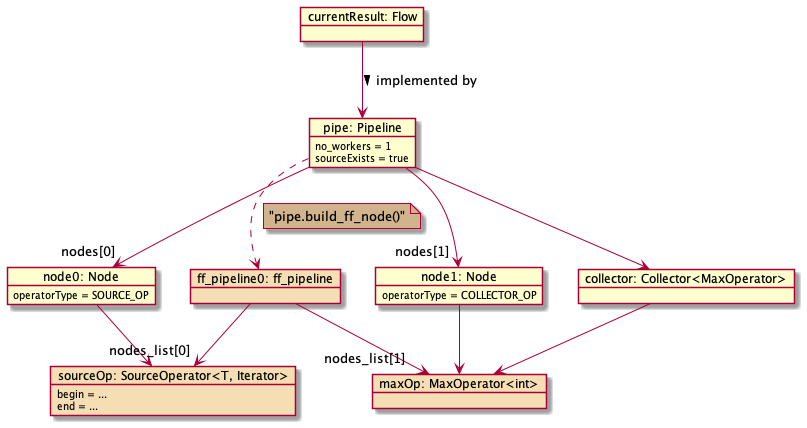
\includegraphics[width=0.66\textwidth]{Figures/objets1-ff.png}
      \caption{La structure interm\'ediaire \TT{PpFf} et le graphe FastFlow associé pour l'exemple~1.}
       \label{objets1-ff.fig}
\end{figure}

\TT{PpFf} construit tout d'abord une repr\'esentation interm\'ediaire, puis g\'en\`ere ensuite un graphe de n\oe{}uds \TT{FastFlow}. La repr\'esentation interm\'ediaire, illustr\'ee dans la figure~\ref{objets1-ppff.fig}, est compos\'ee d'objets de type \TT{Pipeline} et \TT{Node}. Le premier objet cr\'e\'e est \TT{pipe}, une instance de la classe \TT{Pipeline}. Au fur et \`a mesure que les m\'ethodes sont enchain\'ees dans le \TT{Flow}, \TT{PpFf} construit la structure en ajoutant au \TT{Pipeline} des instances de type \TT{Node}. On peut observer que pour les deux m\'ethodes enchain\'ees dans \TT{Flow}, deux instances du type \TT{Node} sont ajout\'ees au \TT{Pipeline} : \TT{node0} et \TT{node1}. 

Selon l'opération indiquée, chaque \TT{Node} garde une r\'ef\'erence \`a une instance de la classe \TT{Operator}. Dans notre cas, les deux objets \TT{Operator} sont \TT{sourceOp}, une instance de la classe \TT{SourceOperator}, et \TT{maxOp}, une instance de la classe \TT{MaxOperator}. 



\'Etant donn\'e que le dernier op\'erateur du {pipeline}, \TT{maxOp}, est un op\'erateur de type collecteur, cela lance la construction du graphe \TT{FastFlow} associ\'e via la m\'ethode \TT{build\_ff\_node()}. Illustr\'ee dans la figure~\ref{objets1-ff.fig}, la structure \TT{FastFlow} est cr\'e\'ee en parcourant chaque \TT{Node} de la structure interm\'ediaire. 
%
Les objets composant la structure interm\'ediaire se distinguent de ceux composant le graphe \TT{FastFlow} par une couleur diff\'erente~: p\^ale pour les objets \TT{PpFf} et fonc\'e pour les objets \TT{FastFlow}. Soulignons que cette même distinction au niveau des couleurs se retrouve aussi dans les autres exemples. 

Toujours dans la figure~\ref{objets1-ff.fig}, on peut noter que l'appel à \TT{build\_ff\_node()} pour l'objet \TT{pipe} g\'en\`ere un objet \TT{ff\_pipeline}, un objet FastFlow, et que les deux instances de \TT{Node} retournent les op\'erateurs associés, \TT{sourceOp} et \TT{maxOp}, qui sont d'objets de type \TT{ff\_node}, la classe de base d'un graphe \TT{FastFlow}. La structure ainsi cr\'e\'ee sera ex\'ecut\'ee automatiquement en appelant la méthode \TT{run\_and\_wait\_end()} de FastFlow, et le r\'esultat du traitement, dans ce cas l'élément maximum, sera retourn\'e au \TT{Pipeline} par l'interm\'ediaire de l'objet \TT{collector}. 

 
\subsection{Exemple~2~: Un flux simple avec parallélisme de données}

\begin{lstlisting}[
label={objets2.c++},
language=c++,
gobble=4,
caption={Le code source d'un flux pour trouver le maximum d'une collection de données en utilisant les instances parall\`eles d'un \TT{farm}.},
frame=single,
float]
    std::vector<int> elems = {0, 1, 2, 3, 4, 5, 6, 7, 8, 9};

    int currentResult =
        Flow
        ::source<int>(elems.begin(), elems.end())
        .parallel(2)
        .max<int>();
\end{lstlisting}



Le deuxi\`eme exemple illustre le fonctionnement d'un flux avec parallélisme de données, donc utilisant les instances parall\`eles d'un \TT{farm}. Le code source pour cet exemple est présenté dans le listing~\ref{objets2.c++}. Par rapport au premier exemple, il y a une seule op\'eration de plus, introduite dans le flux par le cha\^inage de la m\'ethode \TT{parallel(2)}, qui indique de r\'epartir les \'el\'ements du flux entre deux (2) travailleurs (\emph{threads}). Plus précisément, cette op\'eration cr\'ee et ajoute une instance du type \TT{Farm} au \TT{Pipeline}. Ceci peut \^etre observ\'e dans la structure interm\'ediaire cr\'e\'ee par \TT{PpFf} et illustr\'ee dans la figure~\ref{objets2-ppff.fig}.



\begin{figure}
\centering
         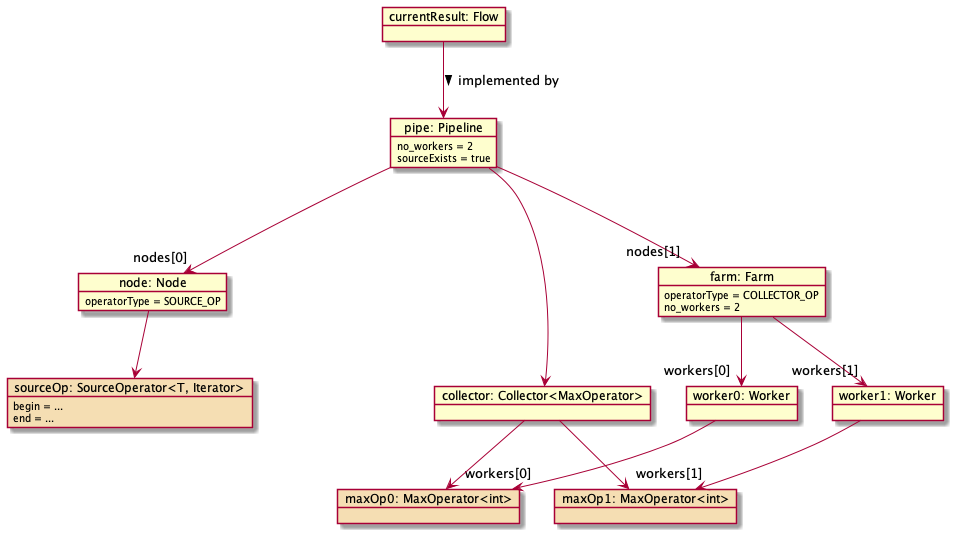
\includegraphics[width=0.6\textwidth]{Figures/objets2-ppff.png}
      \caption{La structure interm\'ediaire \TT{PpFf} pour l'exemple~2.}
       \label{objets2-ppff.fig}
\end{figure}

\begin{figure}
\centering
         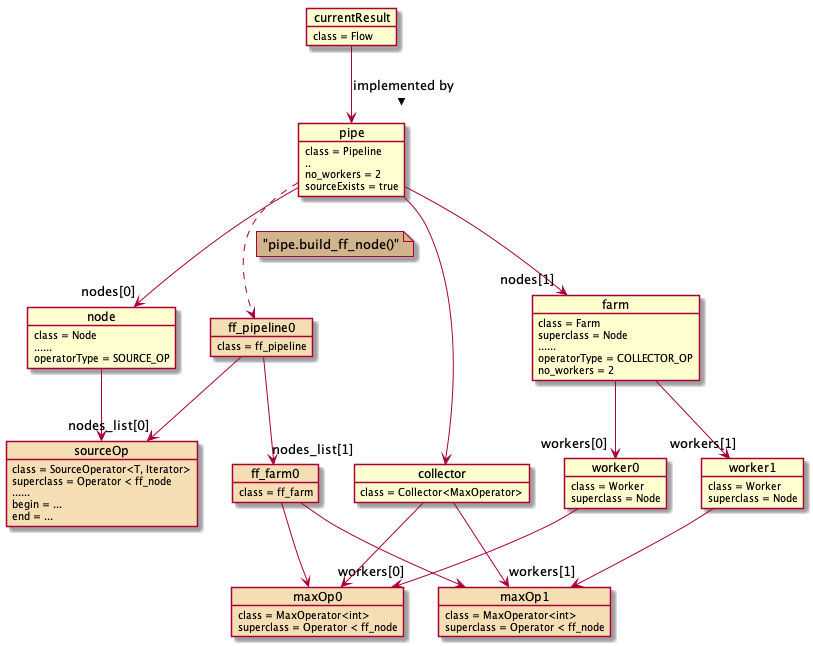
\includegraphics[width=0.6\textwidth]{Figures/objets2-ff.png}
      \caption{La structure interm\'ediaire \TT{PpFf} et le graphe FastFlow associ\'e pour l'exemple~2.}
       \label{objets2-ff.fig}

\end{figure}



On rappelle que lorsqu'une instance de \TT{Farm} est ajout\'ee au {pipeline}, le flux est divis\'e en sous-flux --- appel\'es les instances parall\`eles d'un \TT{farm} --- o\`u chaque sous-flux est une instance de la classe \TT{Worker}. Dans notre exemple, les deux sous-flux sont représent\'es dans la figure~\ref{objets2-ppff.fig} par les instances \TT{worker0} et \TT{worker1}, o\`u chacune de ces instances garde une r\'ef\'erence \`a un objet du type \TT{MaxOperator}. 


\begin{lstlisting}[
label={Collector.c++},
language=c++,
gobble=4,
caption={Le code source de la classe \TT{Collector} qui combine les r\'esultats partiels de chaque sous-flux via la m\'ethode \TT{value()}.},
frame=single,
float]
    template< typename Operator >
    class Collector {
    public:
        Collector(std::vector<Node*> &nodes) : myNodes(nodes)
        {}
        
        Operator::Value value() {
            for (unsigned int i = 1; i < this->myNodes.size(); i++) {
                *((Operator*) myNodes[0]->op()) += 
                *((Operator*) myNodes[i]->op());
            }

            return ((Operator*) myNodes[0]->op())->value();
        }

    private:
        std::vector<Node*>& myNodes;
    };
\end{lstlisting}


On a vu dans l'exemple~1 que lorsqu'un op\'erateur de type collecteur, \TT{maxOp} dans notre cas, est ajout\'e au {pipeline}, ceci lance la construction du graphe \TT{FastFlow} associ\'e via la m\'ethode \TT{build\_ff\_node()}. Illustr\'ee dans la figure~\ref{objets2-ff.fig}, le graphe ainsi g\'en\'er\'e est compos\'e des objets \TT{ff\_pipeline}, \TT{ff\_node} et \TT{ff\_farm} correspondant aux instances de \TT{PpFf} \TT{pipe} (classe \TT{Pipeline}), \TT{sourceOp} (classe \TT{Node}) et \TT{farm} (classe \TT{Farm}). La nouvelle structure cr\'e\'ee sera ex\'ecut\'ee en appelant la m\'ethode \TT{run\_and\_wait\_end()} de \TT{FastFlow}. 

Une différence par rapport \`a l'exemple~1 est que l'instance de \TT{Farm} divise le flux en deux sous-flux et les maximums produits par les sous-flux sont ensuite combin\'es par l'objet \TT{collector}. Ceci est illustr\'e dans la figure~\ref{objets2-ff.fig}, o\`u le \TT{collector} garde une r\'ef\'erence aux deux op\'erateurs, \TT{maxOp1} et \TT{maxOp2}, qui d\'eterminent le maximum pour chaque sous-flux. La combinaison des r\'esultats par le \TT{collector} se fait par l'interm\'ediaire de l'opérateur~<<\TT{+=()}>>. Le code source pour la classe \TT{Collector} est pr\'esent\'e dans le listing~\ref{Collector.c++}. Lorsque la m\'ethode \TT{value()} de cette classe est appel\'ee, les valeurs associées aux op\'erateurs, une pour chaque sous-flux, sont combin\'ees avec l'opérateur \TT{+=()} associé à ce type d'opérateur, et le r\'esultat final (conservé alors dans le n\oe{}ud 0, \TT{myNodes[0]}) est retourn\'e.




\subsection{Exemple~3~: Un flux avec une transformation et avec deux niveaux de parallélisme de données}


\begin{lstlisting}[
label={objets3.c++},
language=c++,
gobble=4,
caption={Le code source d'un flux pour trouver le maximum d'une collection de données en utilisant un nombre de travailleurs distincts.},
frame=single,
float]
    std::vector<int> elems = {0, 1, 2, 3, 4, 5, 6, 7, 8, 9};

    int currentResult =
        Flow
        ::source<int>(elems.begin(), elems.end())
        .parallel(2)
        .map<int, int>(([](int *in){ *in *= 3; return in; }))
        .parallel(4)
        .max<int>();
\end{lstlisting}

Le dernier exemple illustre le fonctionnement du parallélisme de données en utilisant deux s\'eries de \TT{farm}. Le code source est présenté dans le listing~\ref{objets3.c++}. Les deux s\'eries de \TT{farm} sont introduites dans le flux en encha\^inant des appels à la m\'ethode \TT{parallel()}, l'un avec l'argument~2, l'autre avec~4, indiquant que les \'el\'ements du flux doivent être r\'epartis entre deux (2) et quatre (4) travailleurs (\emph{threads}). Par rapport à l'exemple~2, une autre opération de transformation a aussi \'et\'e ajout\'ee au flux, \TT{map}, ici qui multiplie chaque \'el\'ement du flux par la valeur 3.



\begin{figure}
\centering
         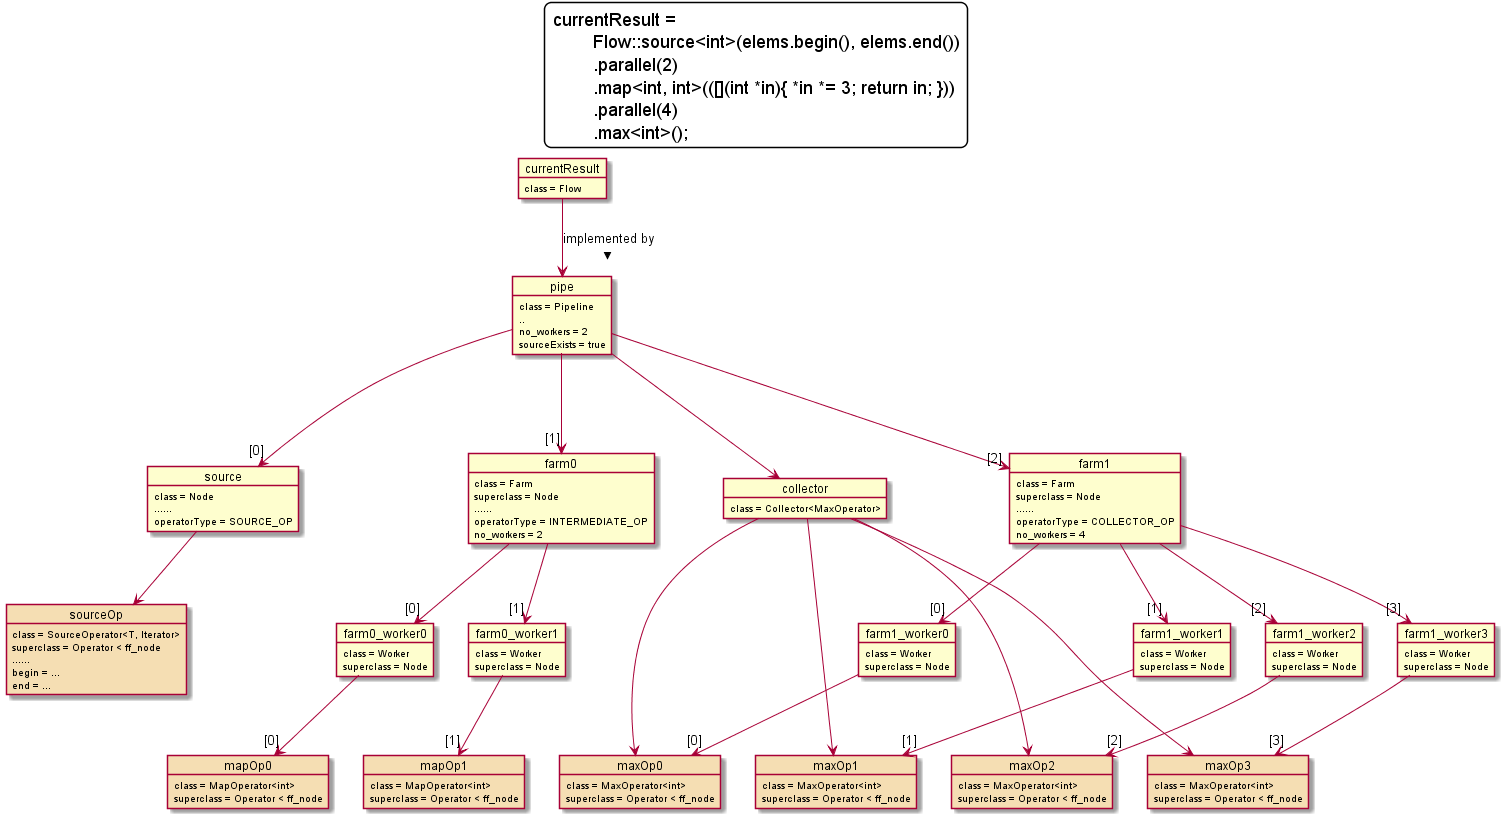
\includegraphics[width=1.0\textwidth]{Figures/objets3-ppff.png}
      \caption{La structure interm\'ediaire \TT{PpFf} pour l'exemple~3.}
       \label{objets3-ppff.fig}
\end{figure}

\begin{figure}
\centering
         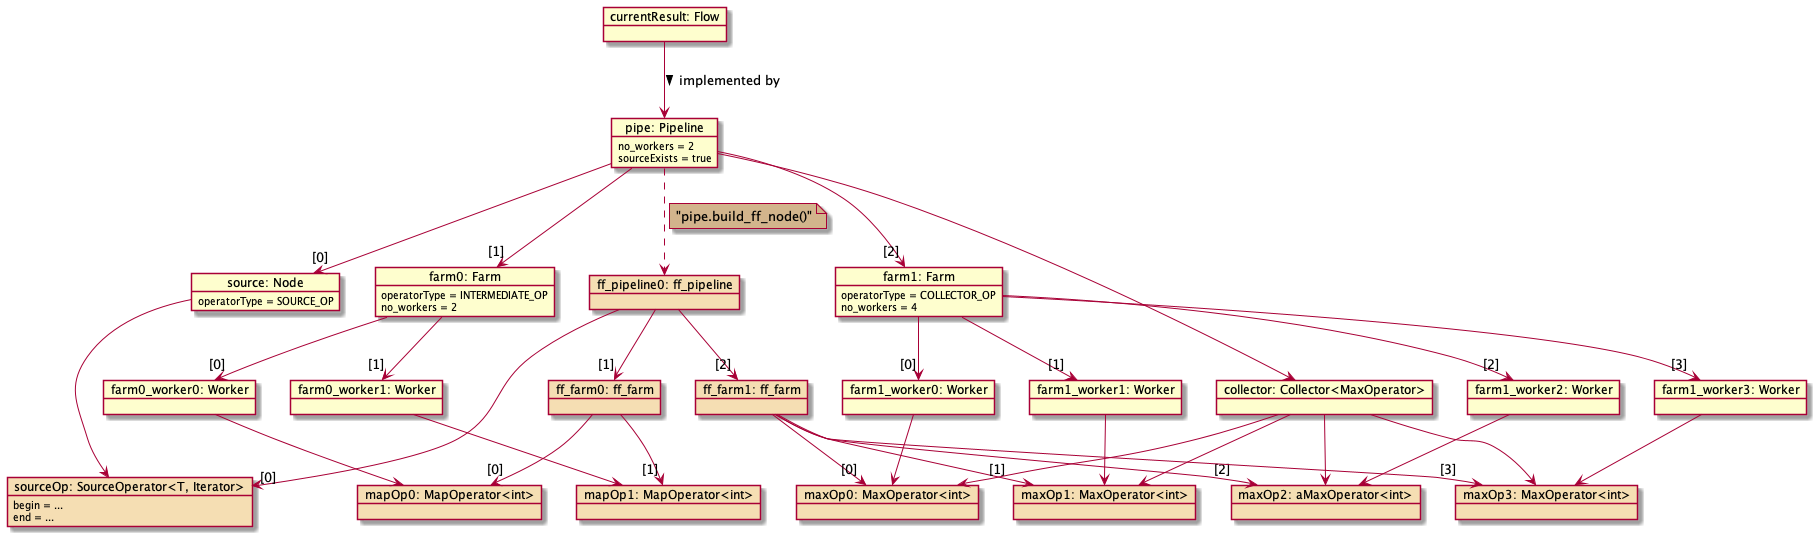
\includegraphics[width=1.0\textwidth]{Figures/objets3-ff.png}
      \caption{La structure interm\'ediaire \TT{PpFf} et le graphe FastFlow associ\'e pour l'exemple~3.}
       \label{objets3-ff.fig}
\end{figure}



La structure interm\'ediaire cr\'e\'ee par \TT{PpFf}, figure~\ref{objets2-ppff.fig}, contient deux instances du type \TT{Farm}, \TT{farm0} et \TT{farm1}. On rappelle que toutes les op\'erations suivant la m\'ethode \TT{parallel}sont ex\'ecut\'ees en parall\`ele dans des sous-flux distincts. Dans notre cas, les op\'erations introduites par les m\'ethodes \TT{map} et \TT{max} seront ex\'ecut\'ees en parall\`ele sur diff\'erents sous-flux, par des instances du type \TT{Worker}. Ceci est illustré dans la figure~\ref{objets3-ppff.fig} o\`u chaque \TT{Worker} de l'objet \TT{farm0} garde une r\'ef\'erence \`a un objet de type \TT{MapOperator} et chaque \TT{Worker} de l'objet \TT{farm1} garde une r\'ef\'erence \`a un objet de type \TT{MaxOperator}. 

Comme dans les deux autres exemples, le graphe \TT{FastFlow} est ex\'ecut\'e apr\'es qu'il est construit via la m\'ethode \TT{build\_ff\_node()}. Ce graphe est illustré dans la figure~\ref{objets3-ff.fig}. Le r\'esultat final, l'\'el\'ement maximum du flux, est d\'etermin\'e par l'objet \TT{collector} en combinant les r\'esultats partiels de chacun de quatre sous-flux de l'objet \TT{farm1}.

